% This document is part of the EPRVCalibration project
% Copyright 2019 the authors. All rights reserved.

% style notes
% -----------
% - use \acronym and use \eprv, \lfc, and so on.

\documentclass[12pt, onecolumn]{aastex63}
\usepackage{xcolor}
\newcommand{\lz}[1]{\textcolor{orange}{#1}}

\usepackage[ruled,vlined]{algorithm2e}
\usepackage{graphicx}

% typesetting words
\newcommand{\project}[1]{\textsl{#1}}
\newcommand{\name}{\project{Excalibur}}
\newcommand{\acronym}[1]{{\small{#1}}}
\newcommand{\expres}{\project{\acronym{EXPRES}}}
\newcommand{\eprv}{\acronym{EPRV}}
\newcommand{\lfc}{\acronym{LFC}}
\newcommand{\code}[1]{\texttt{#1}}

% math shih
\newcommand{\mps}{\mathrm{m\,s^{-1}}}

% margins and page setup, etc
\addtolength{\textheight}{1.00in}
\addtolength{\topmargin}{-0.50in}
\sloppy\sloppypar\raggedbottom\frenchspacing

\begin{document}
\title{\name:
A Non-Parametric, Hierarchical Wavelength-Calibration Model for a Precision Spectrograph}

\correspondingauthor{Lily Zhao}
\email{lily.zhao@yale.edu}

\author[0000-0002-3852-3590]{Lily Zhao}
\affil{Yale University, 52 Hillhouse, New Haven, CT 06511, USA}

\author[0000-0003-2866-9403]{David W. Hogg}
\affil{Center for Cosmology and Particle Physics, Department of Physics, New York University, 726 Broadway, New York, NY 10003, USA}
\affil{Center for Data Science, New York University, 60 Fifth Avenue, New York, NY 10011, USA}
\affil{Max-Planck-Institut für Astronomie, Königstuhl 17, D-69117 Heidelberg, Germany}
\affil{Flatiron Institute, Simons Foundation, 162 Fifth Avenue, New York, NY 10010, USA}

\author[0000-0001-9907-7742]{Megan Bedell}
\affil{Flatiron Institute, Simons Foundation, 162 Fifth Avenue, New York, NY 10010, USA}

\author[0000-0003-2221-0861]{Debra A. Fischer}
\affil{Yale University, 52 Hillhouse, New Haven, CT 06511, USA}

\begin{abstract}
\name\ is a hierarchical, non-parametric framework for wavelength calibrating precision spectrographs.  This method capitalizes on recent hardware improvements in highly-stabilized, extreme-precision radial-velocity spectrographs.  With stabilized spectrographs, the full optical system and detectors can only vary within a tiny range of configurations.  This allows us to use all calibration data to determine the entire space of possible calibrations for a stabilized spectrograph.  A wavelength solution then need only pinpoint where in this low-dimensional calibration space the spectrograph exists.  \name\ also takes advantage of the development of laser-frequency combs or etalons, which generate a dense set of stable calibration points.  This density of points permits the freedom of a non-parametric wavelength solution that can match or adapt to any instrument or detector oddities, more so than any one polynomial.  We demonstrate the success of this method with data from the EXtreme PREcision Spectrograph, \expres, which includes a Menlo Systems laser frequency comb.  We find that \name\ returns more accurate wavelength predictions by more than a factor of 2 over classic, non-hierarchical, polynomial solutions.  Employing \name\ wavelengths on \expres\ RV measurements on HD 3651 reduced the RMS of a planet fit by \lz{blah}.
\end{abstract}


% Add official keywords
\keywords{instrumentation: spectrographs -- instrumentation: detectors -- techniques: spectroscopic -- techniques: radial velocities -- methods: data analysis -- methods: statistical}

\section{Introduction} 
Extremely precise, radial-velocity (\eprv) programs have been incredibly fruitful in finding and characterizing extra-solar planets \citep{mayor2011, bonfils2013, plavchan2015, butler2017}.  These programs typically make use of spectrographs with resolutions on the order of $10^5$, which correspond to line widths on the order of $3000\,\mps$.  Exoplanet science happens at the level of $3\,\mps$ precision, with current instruments hoping to reach $0.1\,\mps$ precision \citep{fischer2016}.  This requires new spectrographs to be calibrated or stabilized to better than $10^{-4}$ of a pixel (assuming that the spectrographs are well sampled).    Some hardware--software systems, such as ESPRESSO, \expres\, and NEID were designed to deliver precision at this level \citep{pepe2013,  jurgenson2016, neid}.  Early data from \expres\ and ESPRESSO suggest that the hardware improvements do propagate through to sub-$\mps$ uncertainties on final, on-sky RV measurements \citep{blackman2020, petersburg2020, pepe2020}.

Traditionally, wavelength solutions are constructed by fitting a polynomial to lines from a calibration source to describe the relationship between wavelength and pixel for each echelle order \citep{lovis2007, cersullo2019}.  Each calibration image is treated independently, though the entire set of calibration images has been used to vet incongruous lines \citep{coffinet2019}.  Just recently, work has been done that suggests a segmented polynomial in the dispersion direction, tuned to detector defects, better describes the wavelength solution than a single, continuous polynomial \citep{milakovic2020}.

Here we propose to simplify and improve calibration programs for \eprv\ hardware systems with two very simple but innovative ideas.  The first flows from the observation that calibration sources---which include arc lamps (in some wavelength ranges), etalons, and laser-frequency combs (\lfc s)---illuminate the spectrograph with very stable, very dense sets of lines; almost every location in the spectrograph image plane is surrounded by nearby, useful calibration lines.

This recommends a calibration methodology that is \emph{non-parametric}:  If every point in the spectrograph detector is surrounded by nearby calibration lines, the wavelength solution can, for example, be made simply as an interpolation of the calibration data.  The density of lines removes the need to enforce any functional form for the wavelength solution (such as a continuous eighth-order polynomial, for example).  In some ways, this is a generalization of the recent work that demonstrated the efficacy of constructing a wavelength solution as multiple, segmented polynomials \citep{milakovic2020}.  Going non-parametric will improve calibration accuracy by not forcing the choice of a parametric form that may bias the calibration, especially when the chosen function is inappropriate (as, for example, polynomials will be at detector edges).

The second simple idea follows from the observation that contemporary \eprv\ instruments are incredibly stable.  Temperature-controlled, fiber-fed spectrographs vary only slightly over the night or season, and only along a small number of axes in what you might call ``calibration space'', or the (very high dimensional) space of all possible wavelength solutions.  That is, not only are the spectrographs stable, but they also have few environmentally accessible degrees of freedom.  This renders it inadvisable to fit each calibration exposure or calibrate each science exposure independently.  Instead, all the calibration data (or all the data) should be used to determine the space in which the instrument can and does vary.  Subsequent calibration work then need only determine where in the accessible part of calibration space the spectrograph was located for each exposure.

In the context of probabilistic models, this structure is \emph{hierarchical}:  The calibration data are used not just to determine the wavelength solution, but also to determine the possible \emph{space} of wavelength solutions.  In the statistics literature this concept is often described as \emph{de-noising}:  Every calibration exposure contains information about every other exposure.  Thus every exposure can be improved (i.e. de-noised) with information from every other exposure.

The method we propose here---\name---embodies these ideas.
It is a non-parametric, hierarchical, data-driven model for the wavelength solution.  By being non-parametric, it delivers enormous freedom to the wavelength solution to match or adapt to any instrument or detector oddities.  By being hierarchical, it restricts that freedom tremendously, but it does so appropriately for the empirically exercised variations in the stabilized spectrograph.  \name\ is designed for temperature-controlled, fiber-fed spectrographs with good calibration sources, such as laser-frequency combs, or etalons.  We have in mind the \eprv\ instruments and \eprv\ science cases, but we expect \name\ to have applications for other kinds of spectrographs in other contexts.  The motivating ideas behind this project are true for almost every astronomical spectrograph.

\section{Method} \label{sec:method}
\name\ is designed to turn a series of calibration lines with known wavelengths and well-fit detector positions, and de-noise and interpolate them into a full wavelength model applicable to all exposures taken with the instrument.  \name\ operates on the two core ideas that the wavelength solution should be given enormous flexibility, but that it lives in a very low-dimensional space, where the degrees of freedom are set by the limited kinematics of the stabilized spectrograph hardware.

\name\ assumes dense enough calibration line coverage with well-fit line centers to provide some constraint on an interpolated wavelength solution across an echelle order.  Additionally, \name\ assumes the instrument hardware is stabilized enough that the space of possible calibration states is low-dimensional.

Wavelength calibration is usually posed in the following way.  Given an exposure $n$, and echelle order $m$, there is a relationship between
the two-dimensional $(x,y)$-position on the detector and the
wavelength $\lambda$
\begin{equation}
\lambda(x,y,m,n) = f(x,y,m;\theta_{n})
\quad ,
\label{eq:wsol}
\end{equation}
where $\theta_{n}$ represents the parameters describing a given exposure.

Classically, pipelines employ polynomials to construct smooth wavelength solutions for each exposure.  For example, the \expres\ pipeline sets the function $f(x,m;\theta_{n})$ from Equation \ref{eq:wsol} to be a 2D, 9\textsuperscript{th}-order polynomial where $\theta_{n}$ represents the polynomial coefficients, $c_{nij}$, unique to each exposure $n$ \citep{petersburg2020}.
\begin{equation}
\lambda(x,m,n) = \sum_{i=0}^9\sum_{j=0}^9 c_{nij}\, x^i\,m^j + \mathrm{noise}
\quad ,
\label{eq:poly_wsol}
\end{equation}
where the y-dependence is dropped as that dependence is carried by spectral order $m$.  The coefficients $c_{nij}$ are interpolated to time $t_n$ of exposure $n$ by a third-order polynomial of time.  This third-order polynomial is evaluated at the time of non-calibration exposures to re-construct a 2D, 9th-order polynomial wavelength solution for that exposure.  Each calibration image obtains in $c_{nij}$ coefficients independently.

Given a stabilized instrument, however, the spectrograph should experience only low-degree variability, meaning the calibration of any image can and should be informed by the calibration of every other image.  The calibration data themselves can be used to develop a low-dimensional basis for expressing the space of possible calibrations for a stabilized spectrograph.

If the space of all calibration possibilities is in fact $K$-dimensional (where $K$ is a small integer, i.e 2 or 8 or thereabouts), and if the calibration variations are so small that than can be linearized, then the function $f(x,m;\theta_{n})$ from Equation \ref{eq:wsol} should be low-dimensional.  In \name, we transpose the calibration model---making the position $x$ a function of $\lambda$---into the following form
\begin{equation}
x(\lambda,m,n) = g_0(\lambda,m) + \sum_{k=1}^K a_{nk}\,g_k(\lambda,m)
\quad ,
\label{eq:excl_wsol}
\end{equation}
where
$g_0(\lambda,m)$ is the fiducial or mean or standard calibration of the spectrograph,
the $a_{nk}$ are $K$ scalar amplitudes for each exposure $n$,
and the $g_k(\lambda,m)$ are basis functions expressing the ``directions'' in calibration space that the spectrograph can depart from the fiducial calibration.  When this calibration structure is used to deliver a wavelength solution, we will have to invert $x(\lambda,m,n)$ into $\lambda(x,m,n)$.

The challenge is to learn these basis functions from the data and get the $K$ amplitudes, $a_{nk}$, for every exposure $n$.  There are many ways to discern these basis functions.  In this paper, we present a model using principal component analysis (PCA).  A PCA is justifiable in the limit where there is very high signal-to-noise ratio, as is usually the case with typical calibration images.  There are many alternatives to PCA for this dimensionality reduction; we return to this point in the discussion (\textsection \ref{sec:discussion}) below.

\subsection{Dimensionality Reduction: De-Noising of Calibration Frames} \label{sec:denoising}
Within a given range of stability, \name\ will use calibration images to  1) determine the space in which the instrument varies and 2) where in the accessible calibration space the spectrograph existed for each exposure.  For each calibration exposure, $n$, \name\ requires a full list of lines, $(\lambda,m)$ that are expected in each calibration exposure.  Each line is uniquely defined by a combination of echelle order, $m$, and ``true'' or theoretical wavelength, $\lambda$. 

For each exposure, $n$, every line, $(\lambda,m)$, has an associated fitted detector position, $x(\lambda,m,n)$, for example x-pixel in an 2D extracted echelle order.  Fitted line centers that are missing from an exposure (e.g. because the fit failed due to noise, the line is not in its usual echelle order, etc.) can be assigned a \code{NaN} (hardware not-a-number) for that echelle order instead.  Let there be $M$ lines per exposure.  \name\ reads in a $N \times M$ matrix of line positions for each of $M$ lines for each of $N$ exposures.

The mean of measured line position over the set of calibration exposures represents the fiducial, or standard calibration of the spectrograph, $g_0(\lambda,m)$.  In this implementation of \name\, principal component analysis is performed on the difference between this fiducial calibration and each individual line position.  The returned principal components serve as basis functions,  $g_k(\lambda,m)$, expressing the possible deviations of the spectrograph from this fiducial calibration.  The magnitude of each principal component for each exposure, $a_{nk}$, represents the scalar amplitude of these deviations for each exposure.  \name\ then uses a small number, $K$, of principal components to reconstruct a de-noised version of the line positions as formulated in Equation \ref{eq:excl_wsol}.

Missing line center measurements are replaced with de-noised estimates.  This is done iteratively until the estimates of missing line centers change by less than 0.01\%.  This process can be repeated on line centers deemed as outliers by some metric, to account for lines that may have been mis-identified or mis-fit.  The principal components from the final iteration are used to define the spectrograph's calibration space while the associated magnitudes pinpoint where in that calibration space the spectrograph is located for each calibration exposure.

\begin{algorithm}
\SetAlgoLined
\KwData{line positions $x(\lambda,m,n)$ for each exposure $n$, with wavelengths $\lambda$ and echelle orders $m$}
\KwResult{Low-dimensional calibration space of spectrograph}
\While{change in missing or outlier line centers $>$ 0.01\%}
{
	$g_0(\lambda,m) = \overline{x(\lambda,m,n)}$\;
	find $U, \Sigma, V$ s.t. $U\Sigma V^* = (x(\lambda,m,n)-g_0(\lambda,m))$\;
	let $a_{n,k} = U\cdot \Sigma$ and $g_k(\lambda,m) = V$\;
	$x(\lambda,m,n) = g_0(\lambda,m) + \sum_{k=1}^K a_{nk}\,g_k(\lambda,m)$ where $K=6$ for $x(\lambda,m,n)$ = \code{NaN}
	}
\caption{Dimension Reduction and De-Noising}
\end{algorithm}

\subsection{?Interpolating Calibration Frames?}
 \label{sec:interp_time}
The magnitude of each principal component can be interpolated with respect to housekeeping data, such as time, temperature, telescope position, etc. to determine different calibration states of the spectrograph.  The choice of what to interpolate against depends on the dominant contribution to variation in the instrument.

In the implementation of \name\ presented here, the magnitudes of the principal components are interpolated with respect to time.  New magnitudes $a_n'k$ values are found for the midpoint time of non-calibration exposures and used to construct the calibration state of the spectrograph for that exposure.  Using interpolated magnitudes, $a_{n;k}$ and the basis vectors, $g_k(\lambda,m)$, returned by the de-noising process, \name\ can construct a set of calibration lines, $x(\lambda,m,n') $, for any exposure as prescribed in Equation \ref{eq:excl_wsol}.


\subsection{Interpolating a Wavelength Solution} \label{sec:interp_wsol}
From the de-noising step, \name\ can now construct a set of calibration lines, $x(\lambda,m,n')$ for any exposure $n'$.  To construct a wavelength solution, \name\ then interpolates the known wavelengths over the exposure specific line centers.  For instance, interpolating the known wavelengths vs. line centers onto every integer x will generate wavelengths for each pixel in an echelle order.

\begin{algorithm}
\SetAlgoLined
\KwData{the fiducial calibration of the spectrograph $g_0(\lambda,m)$; magnitudes of the principal components for each exposure $a_{n,k}$; basis vectors spanning the calibration space of the spectrograph $g_k(\lambda,m)$; }
\KwResult{Wavelengths for detector positions $x'(m,n')$ of exposure $n'$ with time $t_{n'}$}

Find $a_{n',k}$ by interpolating $a_{n,k}$ with to $t_{n'}$\;
$x(\lambda,m,n') = g_0(\lambda,m) + \sum_{k=1}^K a_{n'k}\,g_k(\lambda,m)$ where $K=6$\;
\For{each unique $m$}{
	interpolate $\lambda$ with respect to $x(\lambda,m,n')$ onto pixels $x'(m,n')$\;
	}
\caption{Generating Wavelength Solution}
\end{algorithm}


\section{Data} \label{sec:data}
We tested \name\ results using data from \expres\, the EXtreme PRecison Spectrograph.  \expres\ is an environmentally-stabilized, fiber-fed, $R\sim137,000$, optical spectrograph \citep{jurgenson2016, blackman2020}.  \expres\ has two different wavelength calibration sources, a ThAr lamp and a Menlo Systems laser frequency comb (LFC, e.g. \cite{wilken2012, molaro2013, probst2014}).

Rather than using a simultaneous calibration fiber, two to three LFC exposures are interspersed between science exposures every 15-30 minutes.  ThAr exposures are taken at the beginning and end of each night.  All calibration data is taken through the science fiber, meaning they traveling down the same optical pathway and are projected onto the same pixels as all science observations.

The results and discussion presented here are based off of 1227 LFC exposures taken between October 14 and December 18, 2020 on 29 unique nights.  LFC lines cover 40 echelle orders, which contain 19203 lines.  Though the results are primarily based on work with LFC data, there is some discussion of applications to arc lamps.  These results use 78 ThAr exposures that were taken on the same nights.  ThAr lines cover all 86 extracted orders of \expres, which includes 5295 lines.  For both the LFC and ThAr data, lines that appeared in less than 60\% of exposures were not included in the analysis.  Similarly, files with more than 60\% of expected lines missing were cut from the analysis.  

 \name\ proceeds from a given list of echelle orders, line wavelengths, and pixel positions of each line for each exposure.  We, therefore, use line positions generated by the pre-existing \expres\ pipeline \citep{petersburg2020}.
 
 A ThAr wavelength solution is generated from each ThAr exposure using the IDL code \texttt{thid.pro}, developed by Jeff Valenti.  This code identifies ThAr lines by matching lines in an exposure against a line atlas. 
 
 Flat-relative, optimally extracted LFC data is background-corrected using a univariate spline.  Each peak in an echelle order is then fit to a Gaussian.  The mean of the fitted Gaussian is taken to be the center of the line.  For each line, the ThAr wavelength solution is used to estimate the mode number of a line.  The precise wavelength is then calculated using
 \begin{equation}
 f_n = n \times  f_r + f_0
 \label{eq:lfc}
 \end{equation}
 where the repetition rate, $f_r$, is known from design of the LFC, and the offset frequency, $f_0$, has been determined experimentally.  the pre-existing \expres\ pipeline then generates wavelength solutions on a night-by-night basis as described in Section \ref{sec:method}.
 
 \lz{(Mention degeneracy with prescribed line center and wavelength solution here?  Or in discussion?)}
 
In order to satisfy the assumption of stability needed for \name, only exposures from only one ``instrumental epoch" of \expres\ are used.  \expres\ exposures are separated into different instrumental epochs that correspond to atypical hardware changes--changes that altered the position of the echellogram on the detector, the shape of the instrumental PSF, or the calibration sources.  Significant instrumental changes break the assumption of a stabilized instrument with only low-dimensional variations.  Each instrument epoch is therefore treated independently.


\section{Tests}\label{sec:tests}
We perform a series of tests to validate the performance of \name\ and benchmark \name -generated wavelengths against wavelengths generated by a classic, parametric method.  For all these tests, we generate wavelengths for known calibration lines and compare the predicted wavelength to the assigned wavelength of each line.  This inherently folds in errors in the measured line center of each calibration line, but the contribution to the residuals will be the same across all tests.

To assess the classic, polynomial-driven method of wavelength calibration, we take each LFC exposure and separate the lines into even and odd lines.  We then construct a wavelength solution using only the odd lines and use it to predict wavelengths for the even lines; i.e. a polynomial is fit to just the odd lines and then evaluated at the detector position of the even lines.  We then generate a wavelength solution using only the even lines and use it to predict wavelengths for the odd lines.

To test the interpolation step of \name\ (\textsection \ref{sec:interp_wsol}), we employed \name\ on all LFC exposures with odd lines removed.  The resultant basis vectors, $g_k(x,y,m)$,  and weights, $a_{nk}$, are therefore only informed by the even lines of each LFC exposure.  We then predict wavelengths for the odd lines that had been excluded and compare these predictions to their assigned wavelengths.  This allows us to test how accurately an interpolated wavelength solution can predict wavelengths.

To test the denoising step of \name\ (\textsection \ref{sec:denoising}, \textsection\ref{sec:interp_time}), we employed \name\ on 90\% of all LFC exposures.  This means the basis vectors, $g_k(x,y,m)$,  and weights, $a_{nk}$, were constructed using only information from 90\% of all exposures.  We used the results to predict wavelengths for all the lines in the remaining 10\% of calibration exposures.  This allows us to test how well we can pinpoint the calibration state of the spectrograph using \name.

Histograms of the residuals for each of the above described polynomial, interpolation, and denoising tests (respectively) are shown in Figure \ref{fig:testHists}.  Note that the spread in residuals is much smaller for both the denoising and interpolation tests relative to the results of the polynomial wavelength solutionl.

\begin{figure}[h]
\centering
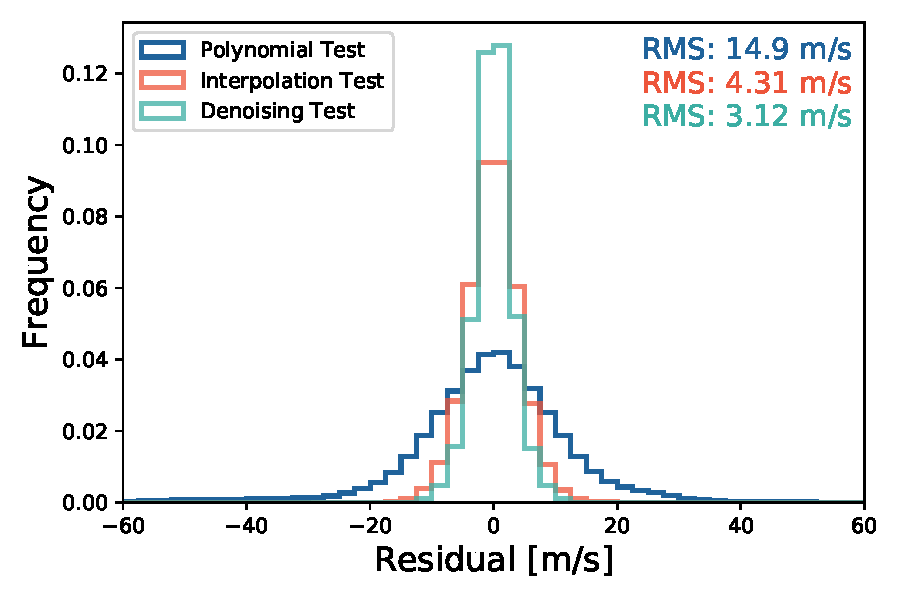
\includegraphics[width=.5\textwidth]{Figures/all_results.pdf}
\caption{Difference in predicted and assigned wavelengths for the wavelength calibration tests described in Section \ref{sec:tests}.  The standard deviation of the residuals for each test is given in the top-right corner in each method's corresponding color.}
\label{fig:testHists}
\end{figure} 

\name -generated wavelengths also exhibit less structure in the returned residuals.  For a randomly selected example LFC exposure, Figure \ref{fig:resid2d} plots each line with respect to its echelle order (y-axis) and x-pixel on the detector (x-axis) colored by the difference between the predicted and assigned wavelength for that line in units of $\mps$.

\begin{figure*}[t]
\centering
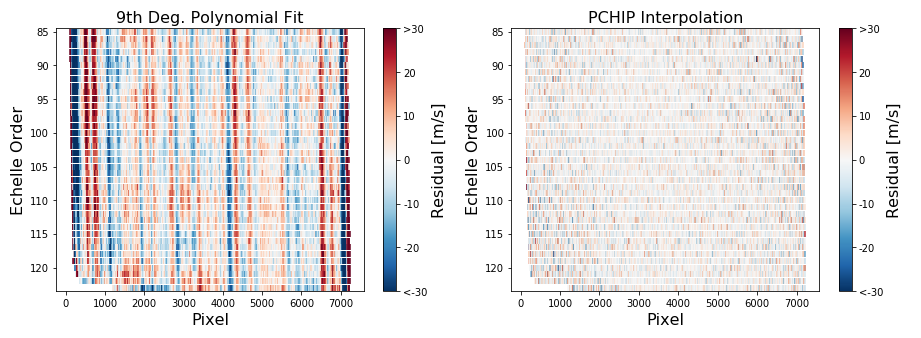
\includegraphics[width=\textwidth]{Figures/lineResids2D.png}
%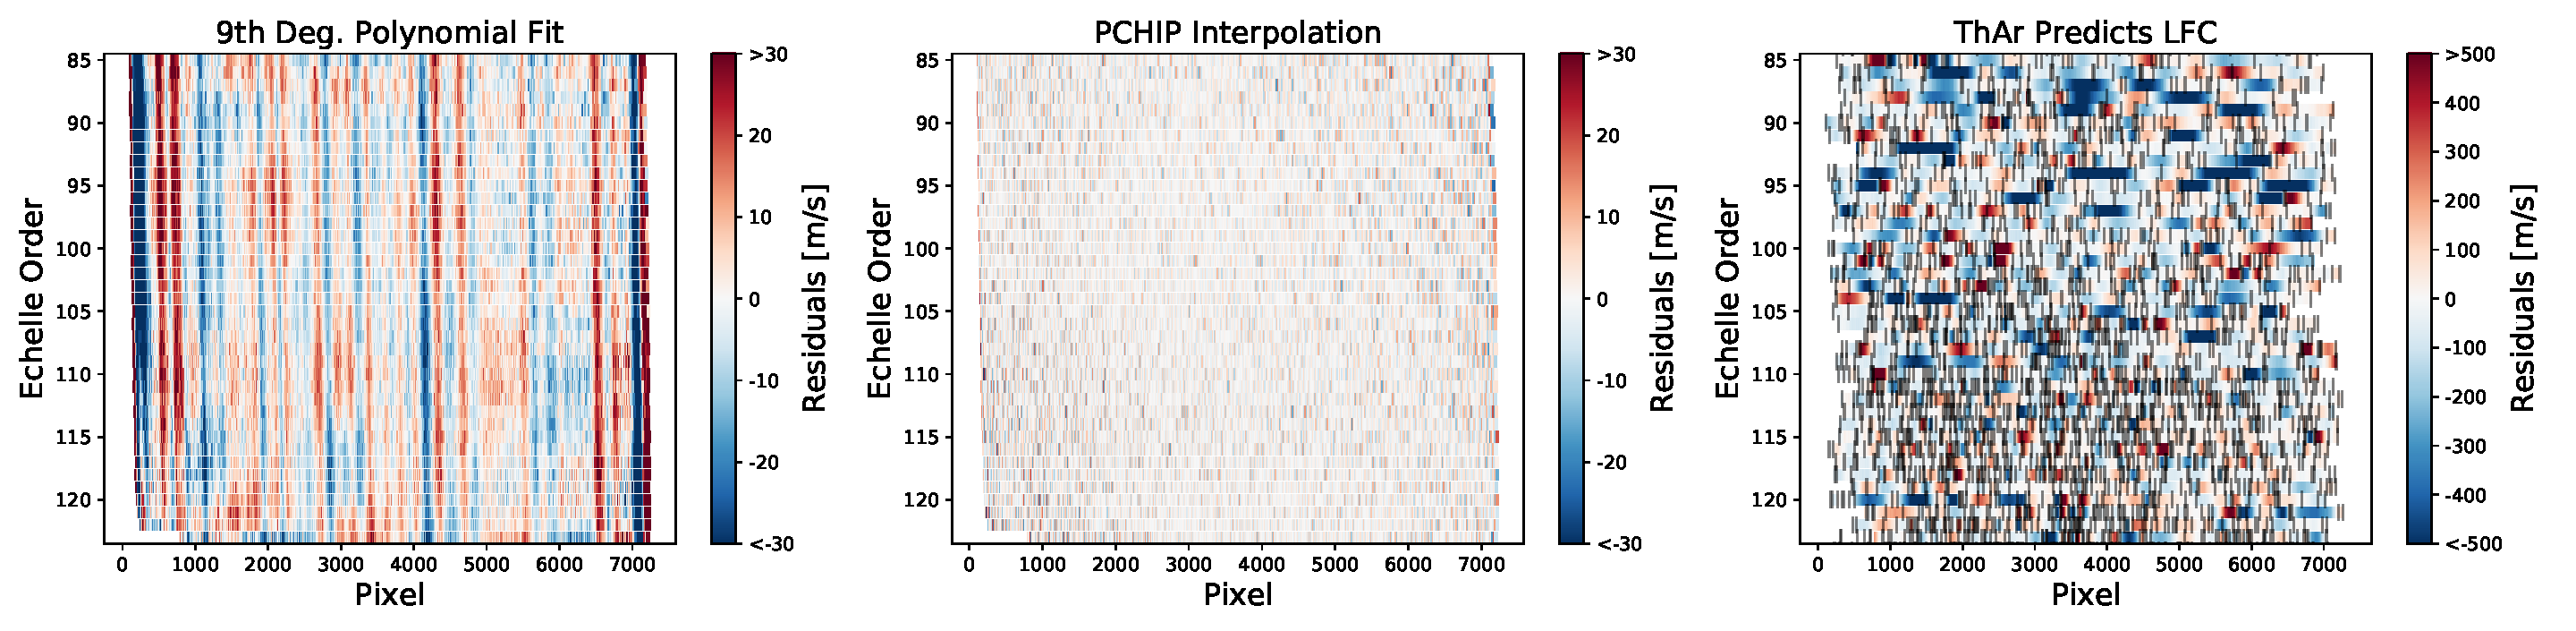
\includegraphics[width=\textwidth]{Figures/lineResids2D.pdf}
\caption{Residuals plotted with respect to detector position (as defined by echelle order and x-pixel) for various wavelength calibration methods.  Each line is colored by the difference between the predicted wavelength and the true wavelength for each line, given in units of $/mps$.  Residuals to a classic, polynomial fit is shown in the left-most plot.  The center plot shows residuals to an interpolated wavelength solution.  The right-most plot shows residuals when a ThAr wavelength solution is interpolated onto LFC line positions.  The position of ThAr lines are over-plotted in black.}
\label{fig:resid2d}
\end{figure*}

\begin{figure*}[t]
\centering
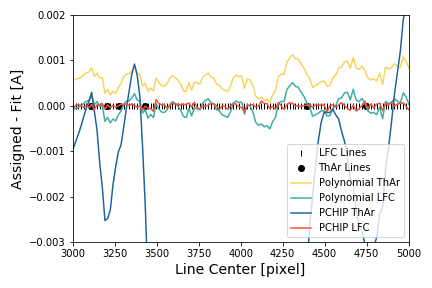
\includegraphics[width=\textwidth]{Figures/lineDensity.png}
\caption{\lz{(Figure I use for talks, maybe shouldn't be included here)}  Comparison of polynomial-fit and interpolated wavelength solutions using either just ThAr lines or LFC lines. Left: the difference between each wavelength solution evaluated at the position of the LFC lines and the assigned wavelength of that LFC line.  The right plot is simply a zoom in of the left plot.  Note the large deviation when trying to implement Excalibur with just ThAr lines, which exhibit much large separations than LFC lines.  The classic, polynomial  fit exhibits similar residuals regardless of whether the set of ThAr lines or LFC lines are used.  Excalibur using LFC lines exhibit the lowest residuals.}
\label{fig:waveResids}
\end{figure*} 

The residuals of the classic, polynomial wavelength solution is shown in the left-most plot of Figure \ref{fig:resid2d}.  There is a lot of vertical structure and some hints of a periodic, diagonal structure as well.

The residuals of the interpolation test for the same exposure is shown in the center plot of Figure \ref{fig:resid2d}.  There is no coherent structure here and smaller residuals.  We believe the flexibility of the interpolated model was able to account for high-order detector defects, which emerged as structure in the residuals of the classic, smooth, polynomial-driven wavelength solution.

The right-most plot of Figure \ref{fig:resid2d} shows the residuals when ThAr exposures, which have much fewer lines than LFC exposures, are run through \name\ and used to predict wavelengths for the completely independent LFC exposures taken during the same range of time.  Over-plotted in black are the positions of the ThAr lines.

Though the interpolated wavelength solution returns lower, less-structured residuals than the polynomial wavelength solution when guided by LFC lines, we see in the right-most plot of Figure \ref{fig:resid2d} that an interpolated wavelength solution can return much worse results in the space between widely separated calibration lines.

The move to an interpolated wavelength solution is driven by the assumption that a high density of calibration lines allows for more freedom in the resultant wavelength solution.  Introducing this flexibility is no longer justified in the regime where there are large spaces between calibration lines, as is the case with a classic ThAr lamp.

Note that running \name\ informed by only ThAr lines cannot be regarded as a direct comparison to the LFC runs, as the increased uncertainty and variability in ThAr line positions alone makes the resultant wavelength predictions an order of magnitude worse, hence the different scale of the colorbar.  All the same, the residuals are relatively worse where lines are further spaced (for example, in redder echelle orders) than where lines are denser.

\subsection{Impact on Radial Velocity Measurements}\label{sec:test-rv}
\lz{Debra and RP currently working through this.  Results seem good.  Will ask them at next group meeting what we should include here}


\section{Choice Choices} \label{sec:choices}
This implementation of \name\ presented here incorporated determining various global variables and methods that we believe are or are close to optimal for constructing a high-fidelity wavelength solution.  This section will describe each choice and the associated decision-making process.

\subsection{Value of K}
The value of $K$ represents the dimensionality of the calibration space within which the spectrograph lives.  In practice, it is the number of principal components, or basis vectors, used to reconstruct the de-noised line centers.  $K$ needs to be large enough so that all variability in the spectrograph is captured.  Too large, however, and the reconstruction will begin to incorporate noise, thereby defeating the purpose.

We settled on a $K$ value of 6.  Figure \ref{fig:pcLfc} shows the first 6 principal components constructed using LFC lines.  In both cases, there is clear structure in the first and second principal components.  The diagonal-banding structure seen in components 3, 5, and 6 we believe to be capturing detector fabrication defects.  Components 3 and 4 show aberrant behavior on the edges of the two bluest echelle orders, where lower signal results in more variation in the line fits.

\begin{figure*}[t]
\centering
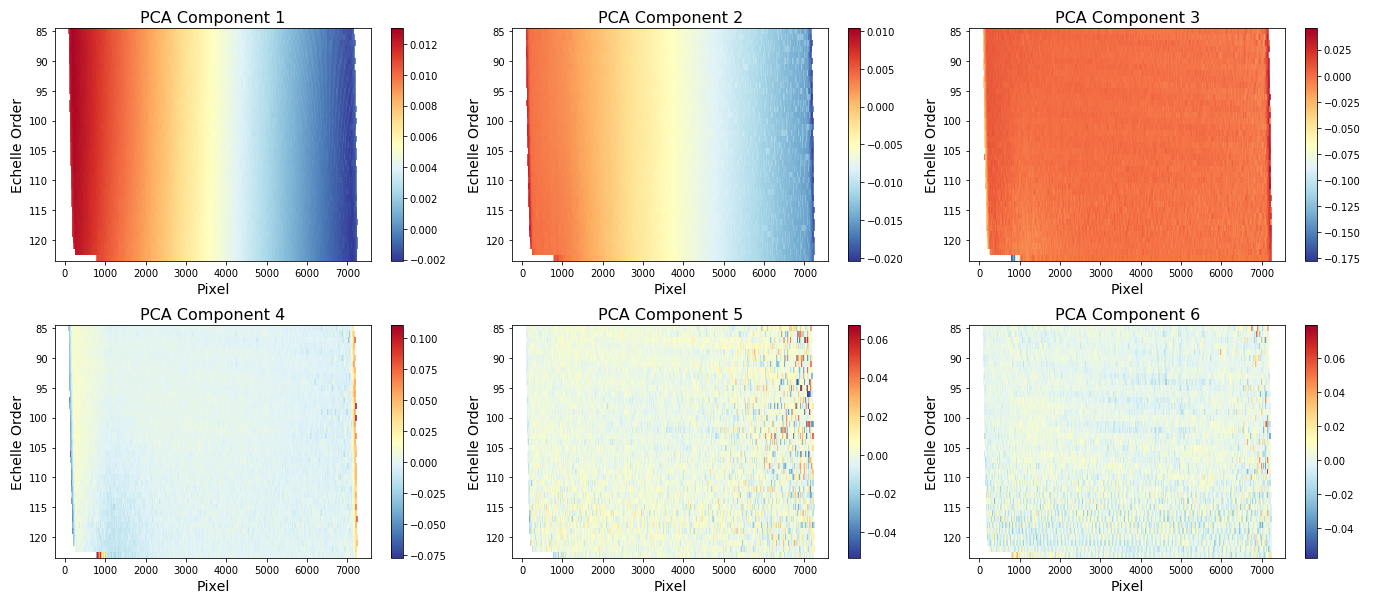
\includegraphics[width=\textwidth]{Figures/pcsLfc6.png}
%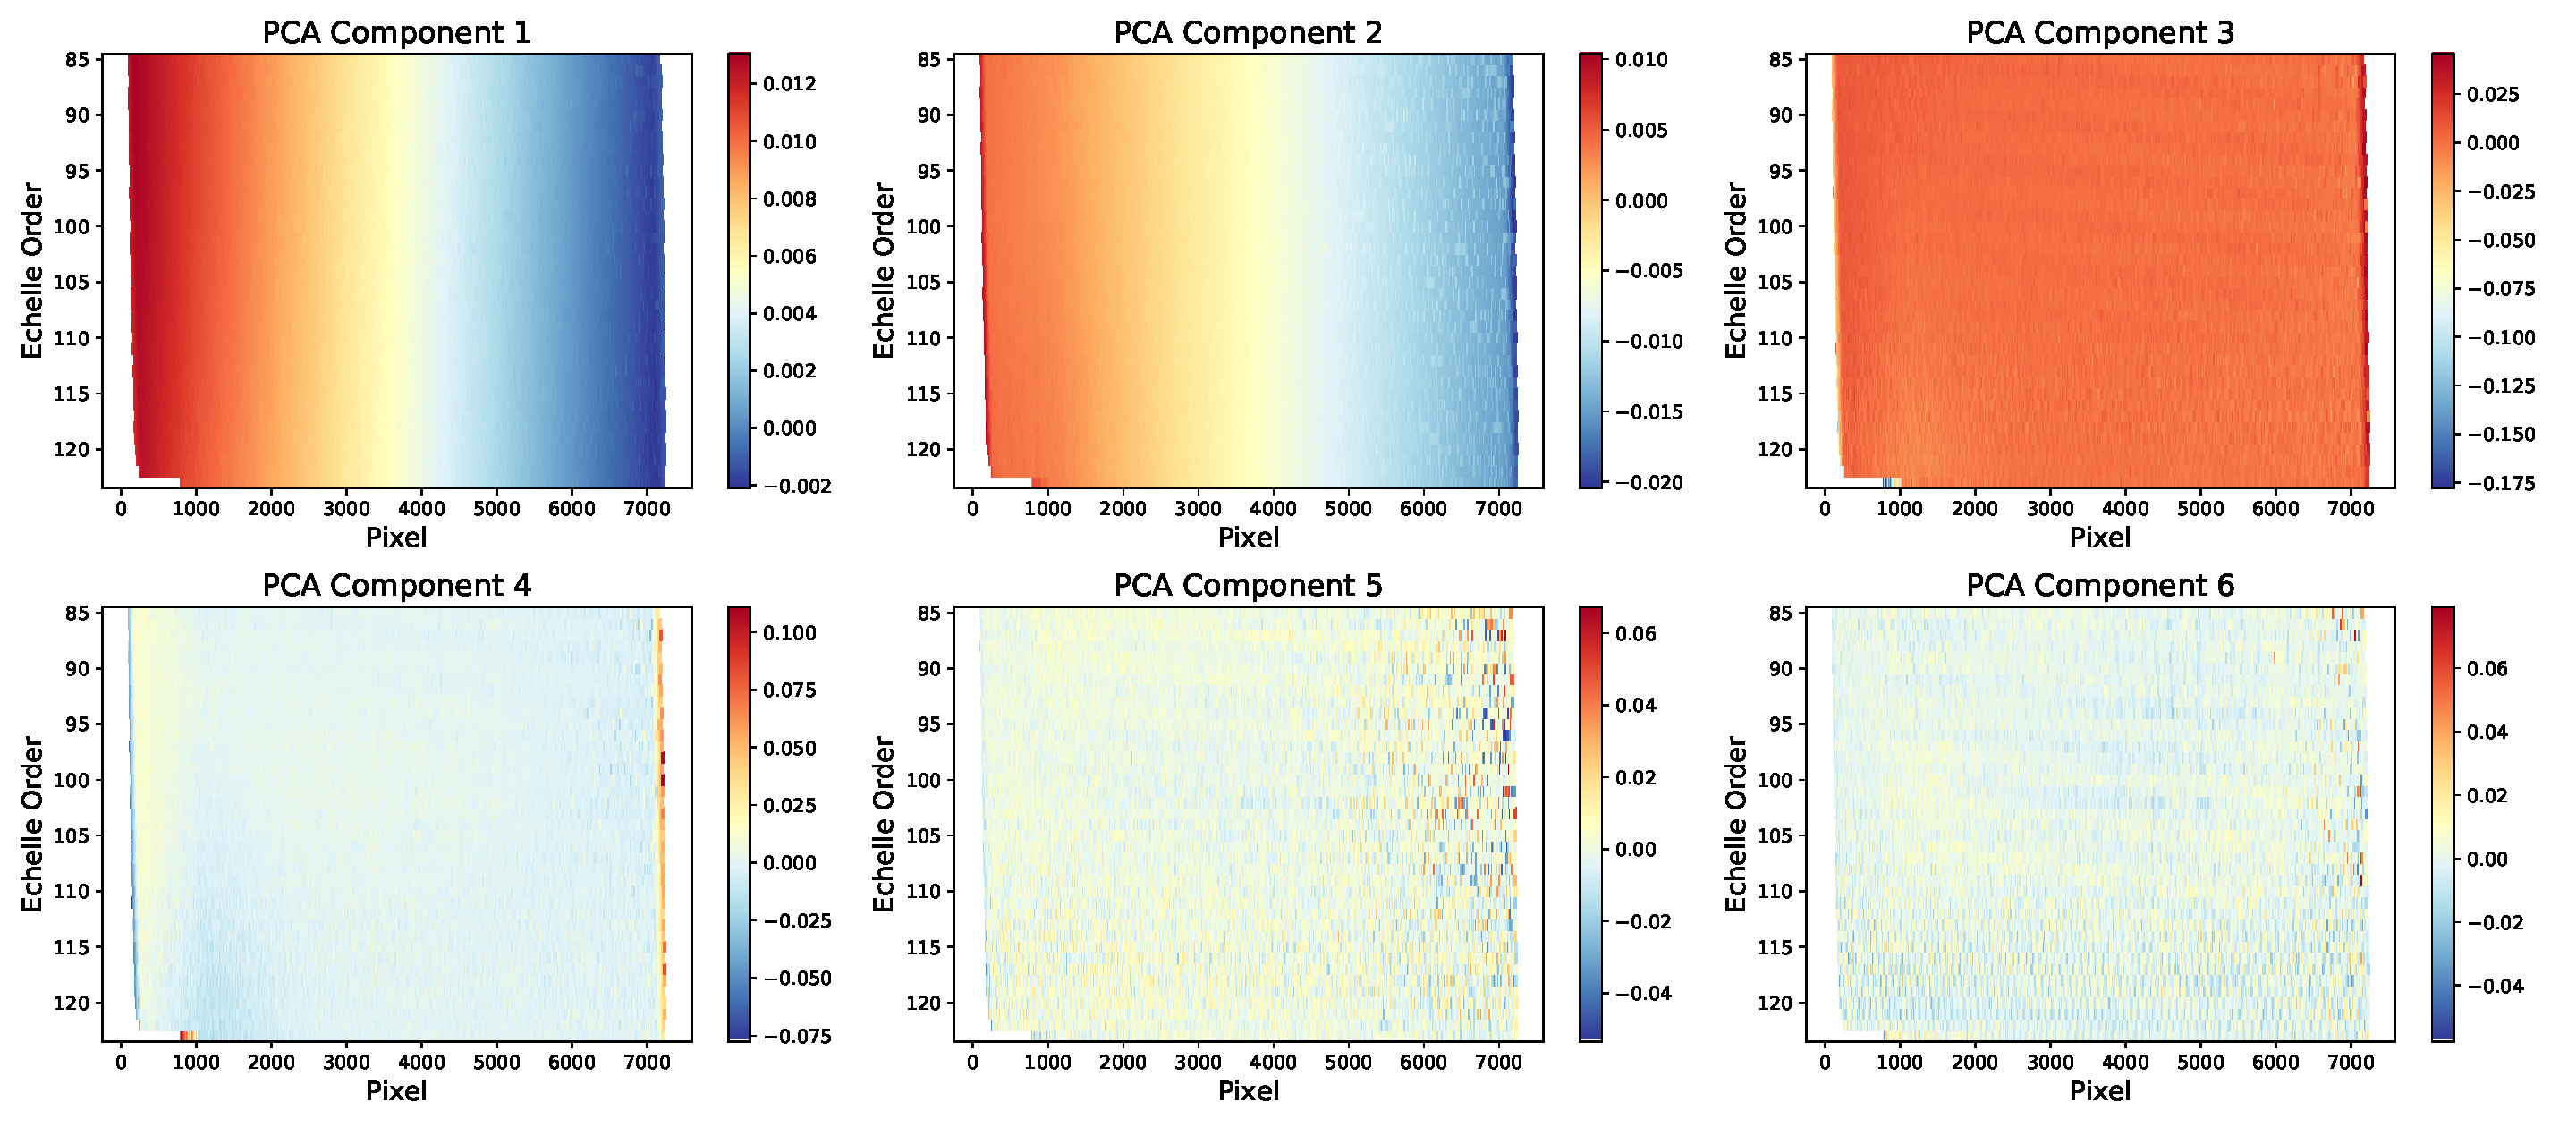
\includegraphics[width=\textwidth]{Figures/pcsLfc6.pdf}
\caption{The first six principal components constructed using LFC lines.  Each line is plotted according to its echelle order and x-pixel and colored by the value of the principal component for that line.}
\label{fig:pcLfc}
\end{figure*}

In deciding a K value, we ran denoising tests, as described in Section \ref{sec:tests}, for K values spanning from 2 to 512.  One would expect the returned wavelengths to get increasingly more accurate with larger K until components that represent only noise are incorporated.  We found that the returned wavelengths have the lowest residuals with a K value of 32.  However, the improvement is slight with K values greater than six.  Comparisons of wavelengths returned by a K=6 model vs. a K=32 model show significant differences for less than 10, bluer lines.  A visual inspection of the principal components, such as the one displayed in Figure \ref{fig:pcLfc}, led us to believe most of the structure is being captured in the first six principal components.

\subsection{Interpolation of $a_{nk}$ with Respect to Time}
Figure \ref{fig:nightlyVariation} shows the amplitude of the first and second principal component with respect to time on the left.  Though there exists a complex overall shape to the amplitudes with respect to time, a clear linear trend exists within each night.  This is shown by the right plots in Figure  \ref{fig:nightlyVariation}.  As the beginning-of-night and end-of-night calibration sets always include LFC exposures, we use a simple linear interpolation to interpolate principal component amplitudes with respect to time.

\lz{Yeah, the right-figure is kind of a mess, isn't it?}

We differentiated eras of stability by where the principal component amplitudes showed large variation.  The analysis was done by eye here, though many algorithms for change-point detection exist in the literature \lz{(Am I going to have to cite things?)}.  We were very conservative with defining eras of stability to ensure that within each era, the calibration-space of the instrument is low-dimensional as assumed.

\begin{figure*}[h!]
\centering
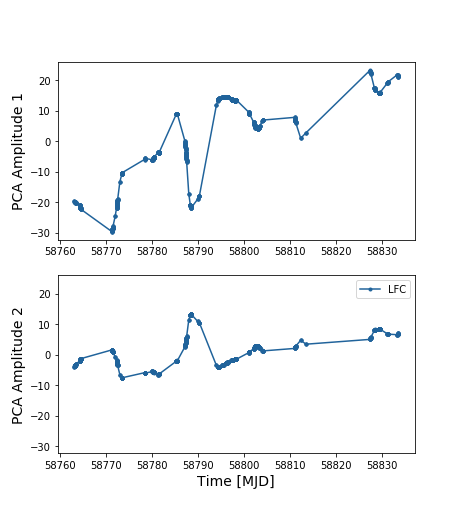
\includegraphics[width=0.56\textwidth]{Figures/pcA_lfc.png}
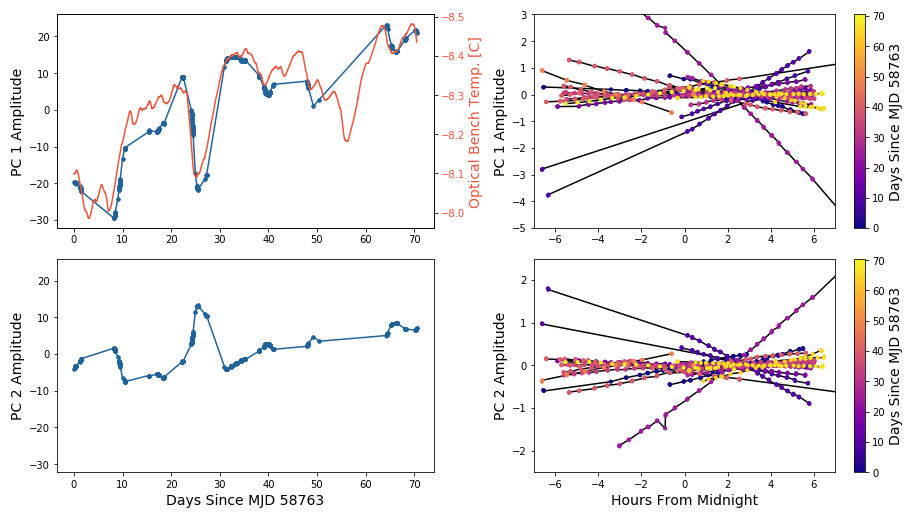
\includegraphics[width=0.42\textwidth]{Figures/pcAs_byDay.png}
\caption{Amplitude of the first two principal components show as a function of time (left) or fraction of a day (right).  The top plots shows the amplitudes for the first principal component while the bottom plot shows the amplitudes for the second principal component.  Points mark the times at which we have calibration data.  Lines show the result of a linear interpolation.  In the right plot, the principal component amplitudes have been artificially offset by the median amplitude for each day so that all days are roughly on the same scale.  Here, points are colored by the MJD of each exposure.}
\label{fig:nightlyVariation}
\end{figure*} 

\subsection{Interpolation of Wavelengths with Respect to Pixel}
Interpolation of wavelengths over pixel  is done order by order using a Piecewise Cubic Hermite Interpolating Polynomial (PCHIP) interpolator.  This interpolation incorporates the flexibility needed to model the changing dispersion of the spectrograph across an echelle order along with any detector defects while also enforcing monotonicity, which we know must be true across any one echelle order.

Due to the dispersion intrinsic to echelle spectrographs, the wavelength change between pixels grows greater with greater wavelengths.  This means that the function of wavelength vs. pixel across an echelle order will always be monotonically increasing and concave down everywhere.  A linear interpolation would obviously give erroneously low values everywhere.

A more classic cubic spline interpolation can run into issues with arc lines, which are irregularly spaced or even blended and can therefore appear very close together.  Very close lines cause huge deviations from the correct wavelengths, as seen in the green line of Figure \ref{fig:xinterp}.

\begin{figure*}[h]
\centering
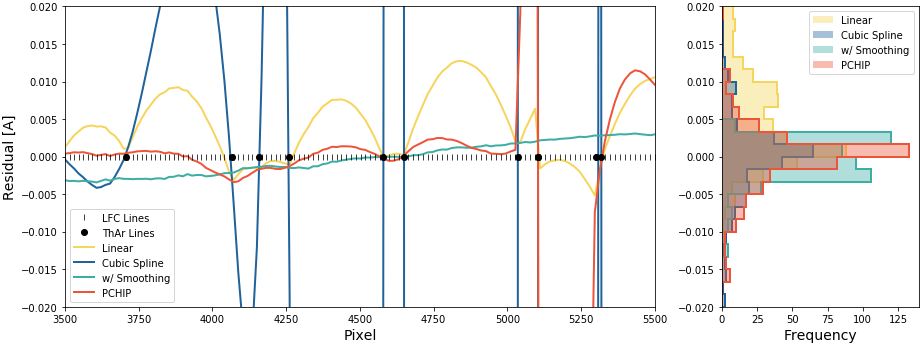
\includegraphics[width=\textwidth]{Figures/intpx_tests.png}
\caption{Results from different interpolation schemes over pixels.  ThAr lines, shown as pink points, are used to construct a wavelength solution that is then evaluated at each LFC line, shown as black lines.  Histograms of the residuals for each method is shown on the right.  Note: there is a blended ThAr line at approximately pixel 5300.}
\label{fig:xinterp}
\end{figure*} 

These huge digressions can be avoided by allowing for some smoothing in the interpolation.  In Figure \ref{fig:xinterp}, we show an example in blue using SciPy's implementation of a univarate spline.  While the result appears to follow the calibration lines much better, the smoothing ultimately causes larger residuals that are spatially correlated (Fig. \ref{fig:xinterp}, right).  In all echelle orders, the edges are overestimated while the middle will be underestimated.  The resultant wavelength solution is underestimating the curvature of the pixel-wavelength relation, giving rise to similar issues as with an inflexible, parametric wavelength solution.  Introducing this smoothing parameter is enforcing a smoothness we have no reason to believe is true of the data.

We instead turn to the PCHIP interpolator, which damps down huge deviations in the traditional cubic spline by requiring the resulting interpolated function be monotonic.  This is a constraint we know is true for any one echelle order.  In Figure \ref{fig:xinterp} we show that using the PCHIP interpolator returns the lowest residuals.

\subsection{Order of Interpolation}
Why do we interpolate in time first and then in x?

\lz{We talked about including this discussion, but there is no real reason for doing things in this order except it is a bit faster.}


\section{Discussion} \label{sec:discussion}
The endeavor to reach $0.1\,\mps$ precision necessitates improvements on all levels of spectroscopy, from the instrumentation to the data analysis.  In this paper, we present \name\, a hierarchical, non-parametric model for wavelength calibration.  

Starting with a list of calibration lines with known wavelengths and well-fit line centers for each calibration exposure, \name\ will de-noise and interpolate the given lines into a full wavelength solution.  We show that \name\ returns residuals with greater than a factor of two less spread than classic, parametric methods.  Using \name\ wavelengths reduced the RMS in a planet fit to derived RVs by \lz{some percent hopefully probs}.

\name\ levies the incredible stability of contemporary EPRV instruments and high density of lines made available by new calibration sources, such as LFCs and etalons, to achieve more accurate wavelengths.  Denser calibration lines allow us to move to more flexible, interpolated wavelength solutions.  Stabilized spectrograph hardware with few degrees of freedom allow us to use all calibration images in a given generation of stability to constrain the accessible calibration space of the spectrograph.

\lz{Choices?}

An advantage of applying PCA to line positions from all LFC exposures is the ability to isolate exposures that exhibit errant variation, which is typically associated with flawed exposures.  This allowed us to quickly vet for problematic LFC exposures, which otherwise would have required visual inspection of all 1200+ LFC exposures.  In a classic framework where each calibration exposure is treated independently, these aberrant exposures would likely have persisted undetected and could potentially sway the resultant wavelength solutions.

On the other hand, the ability of PCA to pick up on any and all variation, regardless of source, also makes \name\ very sensitive to uncertainties in line fitting.  For example, we have seen that lower-signal lines that are harder to fit faithfully will have greater variety in returned line positions, which is in turn captured by the PCA.  High-fidelity line positions are essential to ensure the PCA is capturing variations in the spectrograph's calibration rather than changes in how well a line can be fit.

\name\ can be applied to any data that contains information about the calibration state of the spectrograph.  For example, though LFC and ThAr exposures are used as an example in this paper, \name\ would work exactly the same for an etalon or any other arc lamp with a list of lines and assigned wavelengths.

Furthermore, once we have defined a calibration space that captures all possible degrees of freedom for a stabilized spectrograph, then all exposures taken with the spectrograph contains information about where the spectrograph is located within that calibration space.  Theoretically, science exposures themselves could also be used to determine the calibration state of an instrument, negating the need for any additional wavelength-calibration source beyond defining the calibration space.

We have described only one, fairly simplistic implementation of \name\ here.  There are many options for both the de-noising and interpolation steps.  \lz{(Maybe something to discuss at a future meeting; I'm not actually entirely clear on other possibilities)}.  For instance, a Gaussian process model could be constructed to determine wavelengths in place of a spline. \lz{(?)}  \lz{Something about going Bayesian?}

\lz{(Not sure where this belongs, honestly.)}  We caution that with any wavelength solution, there is a perfect degeneracy between what is defined as the ``center of the line'' and the resultant wavelength solution.  If, for example, a cross correlation method is used to extract RVs from the data, a systematic difference may be introduced depending on the definition of the center of the line.  In principle, the best way to mitigate this uncertainty would be to use a calibration source that looks like a star.

\name\ is designed and optimized for extreme-precision instruments.  We believe that by implementing \name, the uncertainty from wavelength calibration is rendered negligible in the face of other noise sources.


\software{SciPy library \citep{scipy}, NumPy \citep{numpy, numpy2}, Astropy \citep{astropy:2013,astropy:2018}.}

\facilities{LDT}

\bibliography{paper.bib}

\end{document}
